%\usepackage[sc]{mathpazo}
%\usepackage[p]{scholax}
%\usepackage[scaled=1.075,ncf]{newtxmath}
%\usepackage[nomath,variablett]{lmodern}
%\usepackage[usefilenames,DefaultFeatures={Ligatures=Common}]{plex-otf} %
%\usepackage{stickstootext}
%\usepackage[libertine]{newtxmath}
%\usepackage{erewhon}
%\usepackage{times}
%\usepackage[scaled=0.92]{CharisSIL}
%\usepackage[charter]{mathdesign}
%\usepackage{tgschola}
%\usepackage[scaled=1.000,ncf,vvarbb]{newtxmath}
%\usepackage{mathpazo}
%\usepackage[libertine]{newtxmath}

\begin{tikzpicture}
  \begin{axis}[
      axis lines=left,
      axis x line=middle,
      every axis plot post/.style={mark options={fill=black!0, inner sep=0pt}},
      xlabel={$n$},
      ylabel={$\boldsymbol{Amplitude}$},
      ylabel style={
        anchor=north,
        inner sep=5pt,
      },
      xtick={0, 10, ..., 50},
      xmin=0, xmax=55,
      ymin=0, ymax=40,
      xticklabel style={
        anchor=north,
        inner sep=5pt,
      }
    ]
    \addplot [ycomb, black, thick, mark=*] table [x={n}, y={xn}] {medianFilterOriginal.dat};
  \end{axis}
\end{tikzpicture}

\foreach \Point in {(-2,1.5), (-1,1), (-2,3), (-1,2.5), (1,3)}{
    \node at \Point {\textbullet};
}

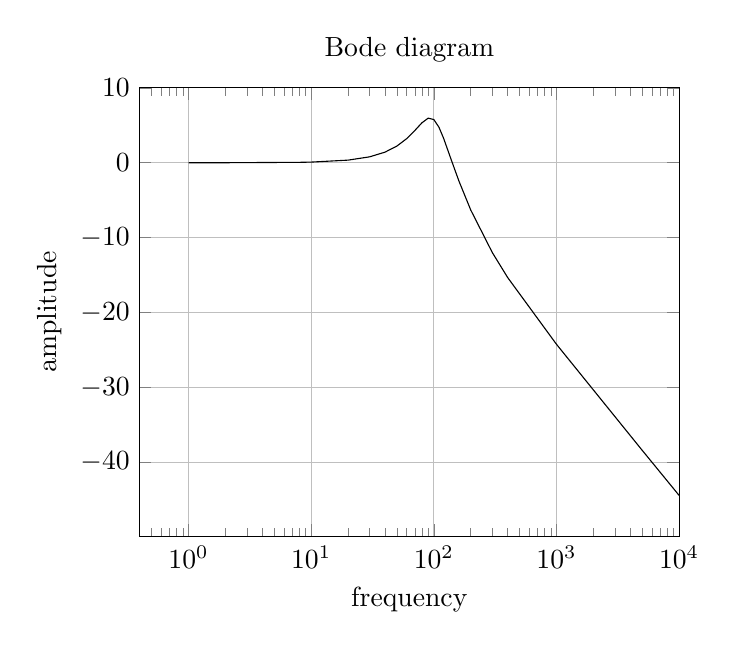
\begin{tikzpicture}
\begin{semilogxaxis}[
title=Bode diagram,
xlabel={frequency},
ylabel={amplitude},
grid=major,
xmax=10^4,
ymax=10]
\addplot[samples at={1,2,8,9,10, 20, 30, 40, 50, 60, 70, 80, 90, 100, 110, 120, 140, 160, 200, 300, 400, 1000, 5000, 6000, 10000}]
{10 * log10( ( (60*x)^2         +(10000)^2 )/
                              ( (-x*x + 10000)^2 + (60*x)^2)
                           )};
\end{semilogxaxis}
\end{tikzpicture}

